\documentclass[12pt]{article}

\usepackage[T1]{fontenc}
\usepackage[letterpaper,margin=1in]{geometry}
\usepackage{graphicx}
\usepackage[hidelinks]{hyperref}
\usepackage{setspace}
\usepackage[table]{xcolor}
\usepackage[dvipsnames]{xcolor}
\usepackage{enumitem}
\usepackage{parskip}
\usepackage{amssymb}
\usepackage{tikz}
\usepackage{listings}
\usepackage{dirtree}
\usepackage{caption}
\usepackage{float}
\usepackage{tabularx}
\usepackage{longtable}
\usepackage{fancyhdr}
\usepackage{titlesec}

\renewcommand*\DTstyle{\ttfamily}
\renewcommand*\DTstylecomment{\rmfamily\color{gray}\small}

\pagestyle{fancy}
\fancyhf{}
\fancyhead[L]{GSoC 2026 | FLARE}
\fancyhead[R]{Lakshit Verma}
\fancyfoot[C]{\thepage}
\renewcommand{\headrulewidth}{0.4pt}
\setlength{\headheight}{15pt}

\definecolor{githubPurple}{HTML}{A371F7}
\definecolor{githubGreen}{HTML}{3FB950}
\definecolor{githubRed}{HTML}{F85149}

% --- Color Definitions for Diagrams ---
\definecolor{greenFill}{HTML}{E8F5E9}
\definecolor{greenStroke}{HTML}{43A047}
\definecolor{memFill}{HTML}{FFF3E0}
\definecolor{memStroke}{HTML}{FFB74D}
\definecolor{coreFill}{HTML}{E1F5FE}
\definecolor{coreStroke}{HTML}{0277BD}
\definecolor{optFill}{HTML}{FCE4EC}
\definecolor{optStroke}{HTML}{E91E63}
\definecolor{procFill}{HTML}{FFF9C4}
\definecolor{procStroke}{HTML}{FBC02D}

\usetikzlibrary{calc, shapes.geometric, arrows.meta, positioning, fit, backgrounds, shadows, shadows.blur, decorations.pathreplacing}

\tikzset{
    dataNode/.style={
        rectangle, rounded corners=3pt,
        draw=greenStroke, thick,
        fill=greenFill,
        minimum width=2.4cm, minimum height=1.2cm,
        align=center,
        drop shadow, font=\sffamily\footnotesize
    },
    memNode/.style={
        cylinder, cylinder uses custom fill,
        cylinder body fill=memFill, cylinder end fill=memFill!90!gray,
        shape border rotate=90,
        aspect=0.25,
        draw=memStroke, thick,
        minimum width=2.0cm, minimum height=1.3cm,
        align=center, drop shadow, font=\sffamily\footnotesize
    },
    opNode/.style={
        rectangle, rounded corners=3pt,
        draw=coreStroke, thick,
        fill=coreFill,
        minimum width=2.6cm, minimum height=1.2cm,
        align=center,
        drop shadow, font=\sffamily\footnotesize
    },
    procNode/.style={
        rectangle, rounded corners=3pt,
        draw=procStroke, thick,
        fill=procFill,
        minimum width=2.6cm, minimum height=1.2cm,
        align=center,
        drop shadow, font=\sffamily\footnotesize
    },
    kernelBox/.style={
        rectangle, rounded corners=8pt,
        draw=coreStroke, thick, dashed,
        fill=coreFill!20,
        inner sep=12pt,
        align=center, font=\sffamily\footnotesize
    },
    group/.style={
        draw=gray!30, dashed, rounded corners=8pt, inner sep=12pt, fill=gray!5
    },
    edgeLabel/.style={
        font=\scriptsize,
        text=black!80,
        align=center,
        inner sep=1pt
    },
    arrow/.style={
        -{Stealth[length=3mm,width=2.5mm]}, thick, color=gray!80
    }
}

\lstdefinelanguage{yaml}{
    keywords={true,false,null,yes,no,on,off,y,n},
    keywordstyle=\color{RoyalBlue}\bfseries,
    ndkeywords={schedule,workflow_dispatch,jobs,strategy,matrix,include,name,runs-on,fail-fast,cron},
    ndkeywordstyle=\color{Plum}\bfseries,
    sensitive=false,
    comment=[l]{\#},
    commentstyle=\color{gray}\itshape,
    moredelim=[l][\color{magenta}]{:},
    morestring=[b]",
    morestring=[b]',
    stringstyle=\color{ForestGreen},
    literate=
     *{-}{{{\color{BrickRed}{-}}}}{1}
      {:}{{{\color{magenta}{:}}}}{1}
      {[}{{{\color{blue}{[}}}}{1}
      {]}{{{\color{blue}{]}}}}{1}
      {\{}{{{\color{blue}{\{}}}}{1}
      {\}}{{{\color{blue}{\}}}}}{1},
    basicstyle=\ttfamily\small
}

\lstdefinelanguage{json}{
    keywords={true,false,null},
    keywordstyle=\color{VioletRed}\bfseries,
    basicstyle=\ttfamily\small,
    showstringspaces=false,
    breaklines=true,
    string=[b]",
    stringstyle=\color{BrickRed},
    literate=
     *      {"file_path":}{{{\color{MidnightBlue}\bfseries "file\_path":}}}{13}
      {"enable_static_strings":}{{{\color{MidnightBlue}\bfseries "enable\_static\_strings":}}}{25}
      {"analysis":}{{{\color{MidnightBlue}\bfseries "analysis":}}}{11}
      {"metadata":}{{{\color{MidnightBlue}\bfseries "metadata":}}}{11}
      {"strings":}{{{\color{MidnightBlue}\bfseries "strings":}}}{10}
      {"qs_enabled":}{{{\color{MidnightBlue}\bfseries "qs\_enabled":}}}{13}
      {"static_strings":}{{{\color{MidnightBlue}\bfseries "static\_strings":}}}{18}
      {"qs_layout":}{{{\color{MidnightBlue}\bfseries "qs\_layout":}}}{12}
      {"string":}{{{\color{MidnightBlue}\bfseries "string":}}}{9}
      {"offset":}{{{\color{MidnightBlue}\bfseries "offset":}}}{9}
      {"encoding":}{{{\color{MidnightBlue}\bfseries "encoding":}}}{11}
      {"qs_tags":}{{{\color{MidnightBlue}\bfseries "qs\_tags":}}}{10}
      {"qs_structure":}{{{\color{MidnightBlue}\bfseries "qs\_structure":}}}{15}
      {"qs_section":}{{{\color{MidnightBlue}\bfseries "qs\_section":}}}{13}
      {"name":}{{{\color{MidnightBlue}\bfseries "name":}}}{7}
      {"length":}{{{\color{MidnightBlue}\bfseries "length":}}}{9}
      {"children":}{{{\color{MidnightBlue}\bfseries "children":}}}{11}
      {:}{{{\color{magenta}{:}}}}{1}
      {,}{{{\color{magenta}{,}}}}{1}
      {\{}{{{\color{blue}{\{}}}}{1}
      {\}}{{{\color{blue}{\}}}}}{1}
      {[}{{{\color{blue}{[}}}}{1}
      {]}{{{\color{blue}{]}}}}{1}
      {0}{{{\color{Plum}{0}}}}{1}
      {1}{{{\color{Plum}{1}}}}{1}
      {2}{{{\color{Plum}{2}}}}{1}
      {3}{{{\color{Plum}{3}}}}{1}
      {4}{{{\color{Plum}{4}}}}{1}
      {5}{{{\color{Plum}{5}}}}{1}
      {6}{{{\color{Plum}{6}}}}{1}
      {7}{{{\color{Plum}{7}}}}{1}
      {8}{{{\color{Plum}{8}}}}{1}
      {9}{{{\color{Plum}{9}}}}{1}
      {.}{{{\color{Plum}{.}}}}{1}
      {-}{{{\color{Plum}{-}}}}{1}
}

\lstdefinestyle{codeblock}{
    frame=single,
    frameround=tttt,
    framerule=0.35pt,
    rulecolor=\color{gray!55},
    backgroundcolor=\color{gray!3},
    breaklines=true,
    showstringspaces=false,
    columns=fullflexible,
    keepspaces=true,
    xleftmargin=0em,
    framexleftmargin=0em
}

\lstset{
    style=codeblock
}

\setstretch{1.15}
\setlength{\parskip}{0.35em}
\setlength{\parindent}{0pt}

\titleformat{\section}{\LARGE\bfseries}{}{0pt}{}
\titleformat{\subsection}{\Large\bfseries}{}{0pt}{}
\titleformat{\subsubsection}{\large\bfseries}{}{0pt}{}

\titlespacing*{\section}{0pt}{1.2ex plus 0.5ex minus 0.2ex}{0.6ex}
\titlespacing*{\subsection}{0pt}{1.0ex plus 0.4ex minus 0.2ex}{0.45ex}
\titlespacing*{\subsubsection}{0pt}{0.8ex plus 0.3ex minus 0.2ex}{0.35ex}

\title{Extend FLOSS to use the rendering techniques pioneered by QUANTUMSTRAND}
\author{Lakshit Verma (\href{https://github.com/vee1e}{vee1e})}
\date{}

\newcommand{\pr}[1]{%
  \href{https://github.com/mandiant/flare-floss/pull/#1}{\textbf{\##1}}%
}

\newcommand{\issue}[1]{%
    \href{https://github.com/mandiant/flare-floss/issues/#1}{\textbf{\##1}}%
}

\begin{document}

\pagenumbering{gobble}

% Title page
\begin{titlepage}
    \centering
    \vspace*{0.5in}
    
\includegraphics[width=0.28\textwidth]{assets/gsoc-logo.png}

    \vspace{0.4in}
    
\includegraphics[width=0.34\textwidth]{assets/flare-logo.png}

    \vspace{0.6in}
    {\LARGE\bfseries Extend FLOSS to use the rendering techniques pioneered by QUANTUMSTRAND\par}
    \vspace{0.35in}
    {\large Lakshit Verma (\href{https://github.com/vee1e}{vee1e})\par}
    \vspace{0.1in}
    {\large \today\par}
\end{titlepage}

\pagenumbering{arabic}

\tableofcontents

\newpage

\section*{Introduction}
\phantomsection
\addcontentsline{toc}{section}{Introduction}

\subsection*{About Me}
\phantomsection
\addcontentsline{toc}{subsection}{About Me}
\begin{tabular}{|p{2.1in}|p{4.4in}|}
\hline
\textbf{Name \& GitHub Handle} & Lakshit Verma (\href{https://github.com/vee1e}{vee1e}) \\
\hline
\textbf{\cellcolor{gray!15}University} & Manipal Institute of Technology \\
\hline
\textbf{\cellcolor{gray!15}Program} & B.Tech in Electrical Engineering (Minor in Computing) \\
\hline
\textbf{\cellcolor{gray!15}Year} & Third Year \\
\hline
\textbf{\cellcolor{gray!15}Graduation} & July 2027 \\
\hline
\textbf{Contact Information} & \href{tel:+918448058867}{+91 8448058867} / vermalucky2004@gmail.com \\
\hline
\textbf{Location / Time Zone} & Mumbai, India / IST (UTC+5:30) \\
\hline
\textbf{Brief CV Link} & \href{https://lverma.com/resume}{\textcolor{RoyalBlue}{\textbf{https://lverma.com/resume}}} \\
\hline
\end{tabular}

\subsection*{Background and Interests}
\phantomsection
\addcontentsline{toc}{subsection}{Background and Interests}

\textbf{What is your background and which current interests do you have?}

I'm Lakshit Verma, an engineering student with a cumulative 2.5 years of experience in the cybersecurity field, mainly through playing Capture The Flag (CTF) tournaments in the reverse engineering and digital forensics domain with my academic team \textbf{\href{https://ctftime.org/team/62713}{Cryptonite}}, ranked as the \#3 Indian CTF team for two consecutive years.
Currently I also serve as a member of the board and the Forensics domain head.
I also possess an open source program background, having been selected for the highly selective \href{https://www.linkedin.com/feed/update/urn:li:activity:7332749666108727296/}{\textbf{C4GT Dedicated Mentoring Program (DMP)}} last year.
It's format is similar to GSoC, occurring over the summer from July to August, a mid-term and end-term evaluation, a mentor guiding you along and reviewing code, and a stipend equivalent to a small-medium GSoC project.
You can see my project from that program \textbf{\href{https://github.com/vee1e/bulk-questionnaire-upload}{here}}; it's a tool to convert XLSForm files to the organization's internal JSON format.
I built the application from scratch, and worked on the Python/FastAPI backend, the Angular JS frontend and the CI/CD GitHub workflows for it.

I have been attended several on-site CTFs, hackathons and security conferences, and won several cybersecurity competitions such as the \textbf{\href{https://www.linkedin.com/posts/lakshitverma_smartindiahackathon2024-teamnitewatch-mitmahe-activity-7273618458590740481-kKHs?utm_source=share&utm_medium=member_desktop&rcm=ACoAAEZUm1oBBRW0ySHd3oHLN9xuTzJSXtxPlv0}{Smart India Hackathon 2024}}, India's largest hackathon, under a cybersecurity problem statement. In it, our team developed a novel parsing methodology to recover deleted data from Linux Btrfs and XFS filesystems, processing raw filesystem images from scratch (from the superblock to individual inodes) with no external libraries included.

I have a strong interest in the FLARE team's tooling for malware analysis and forensics as I've integrated them more in my workflows over the past months, and security tool development is a skill I've been building for the past year through OSS contributions and personal projects.

\textbf{Do you have any background or experience in reverse engineering or malware analysis? If not, why are you interested in learning more about it?}

I have a good amount of experience in reverse engineering, with knowledge and experience of all major decompilers such as Ghidra, IDA Pro, Binary Ninja and Cutter, and supporting tools such as GDB/pwndbg, Speakeasy and WinDbg.

Over the past few years I've designed multiple CTF challenges in the reverse engineering domain, presenting several obfuscation techniques such as a custom VM based obfuscation in niteCTF 2024 (\href{https://github.com/Cryptonite-MIT/niteCTF-2024/tree/main/rev/gate_keeping/solution}{\textbf{writeup link}}) and function hashing and Rust malware in a 3-part incident response series in niteCTF 2025 (\href{https://github.com/Cryptonite-MIT/niteCTF-2025/tree/main/forensics/ir_2_wiege}{\textbf{writeup link}}).

I also possess a good degree of knowledge in the domain of string obfuscation techniques such as runtime decryption, dynamic stack construction, and single and multi-byte XOR encryption, having dealt with the same through an untold amount of crackme's and reverse engineering challenges over the years.

\textbf{As mentors and project coordinators, how can we best support you on your open source journey?}

A mentor's job isn't to simply review code, its to look at the bigger picture of the project, guide the contributor in the right direction, and help them grow as a developer and OSS contributor: enough so that they can not only contribute to but maintain project(s) in the future as well.

My previous experience at C4GT, while insightful, was characterized by mentor apathy and the lack of clear communication and guidance, leading me to work more independently in it. Fortunately I've found the FLARE team and commmunity to be much more available and receptive to newer contributors like me.

Timely, meaningful interactions of mentor and contributor through every step of the way form the backbone of a successful GSoC project, and I hope to have that with you all this summer.

\subsection*{Code Contribution}
\phantomsection
\addcontentsline{toc}{subsection}{Code Contribution}

I have actively contributed to the Mandiant organization over the past three months, with a total of \textbf{\href{https://github.com/pulls?q=is\%3Apr+org\%3Amandiant+author\%3Avee1e+is\%3Amerged}{\textcolor{githubPurple}{11 merged PRs}}} and \textbf{\href{https://github.com/pulls?q=is\%3Apr+org\%3Amandiant+author\%3Avee1e+is\%3Aopen}{\textcolor{githubGreen}{2 open PRs}}} across four repositories: \textbf{flare-floss}, \textbf{flare-floss-testfiles}, \textbf{macOS-UnifiedLogs} and \textbf{stringsifter}. One such contribution is this:

\begin{center}
    \href{https://github.com/mandiant/flare-floss/pull/1221}{\textcolor{RoyalBlue}{\underline{\textbf{PR \#1221: QS: Add Mach-O parsing and samples}}}} \texttt{(\textcolor{ForestGreen}{+566} \textcolor{BrickRed}{-1})}
\end{center}

Wherein I added support for Mach-O structure parsing in QS, which was a major feature addition that resolved a nearly 3 year old issue (\issue{786}) and significantly enhanced the tool's capabilities.

\newpage
\section*{Project Information}
\phantomsection
\addcontentsline{toc}{section}{Project Information}

\subsection*{Project Abstract}
\phantomsection
\addcontentsline{toc}{subsection}{Project Abstract}


QUANTUMSTRAND (QS) is an experiment within FLOSS augmenting traditional output of decoded and deobfuscated strings with context-aware rendering of string metadata to aid in malware analysis, such as the string's location in the binary section, its association with common libraries or APIs through the tagging system. It also contains a GUI viewer providing interactive filtering and visualization of the rendered string data.

With FLOSS being the main tool for string analysis, the end goal of the project is to select the best features from QS and integrate and merge them into the \texttt{master} branch to make them available to the wider reverse engineering community through FLOSS itself. Changes will be made both on the backend and frontend; a new GUI based on the QS viewer will be developed and integrated into the branch as well.

This will involve preliminary research by users of both FLOSS and QS to determine the use cases and features to prioritize, the improvement of the QS codebase to complete some features and get it to a mergeable state, and the actual integration of the features into FLOSS itself.

\subsection*{Project Scope}
\phantomsection
\addcontentsline{toc}{subsection}{Project Scope}

\subsubsection*{In Scope}
\phantomsection
\addcontentsline{toc}{subsubsection}{In Scope}

\begin{itemize}
    \item Improve current QS features to be merge-ready into upstream \texttt{master}.
    \item Implement missing features in QS needed by FLOSS users and developers the most.
    \item Merge the essential features through Incremental Development.
    \item Build a GUI to view extracted FLOSS + QS enhanced strings.
    \item Document such that future developers can build upon the project post GSoC.
\end{itemize}

\subsubsection*{Not in Scope}
\phantomsection
\addcontentsline{toc}{subsubsection}{Not in Scope}

\begin{itemize}
    \item Large, sweeping changes to the QS codebase and their subsequent merging into FLOSS.

    This includes, but is not limited to: new language specific string extraction algorithms, mergers with other FLARE projects such as capa/capa-viewer, and large refactors of the codebase.
\end{itemize}

\subsection*{Detailed description}
\phantomsection
\addcontentsline{toc}{subsection}{Detailed description}


The project will be split into three distinct phases:

\begin{itemize}
    \item \textbf{Improvement of current QS features:} I'm currently working on this with PRs merged such as \pr{1225}, \pr{1229} and \pr{1230}. Completion of issues, both smaller ones like \issue{771} and larger scale ones such as \issue{701} and tag database construction will be the focus of this phase, to ensure the QS codebase is in a workable state and has all the necessary features for integration into FLOSS.
    \item \textbf{Integration of QS features into FLOSS:} This will be the main coding phase where we finalize the features through discussions with the community and the mentor to decide on the ones of priority, and then start slowly introducing them one by one, testing for issues, collecting feedback and repeating from there.
    \item \textbf{Creating an interactive GUI to display strings:} Extend the currently bare-bones GUI in \texttt{quantumstrand/qs-viewer} to a feature complete and FLOSS output interface with all the features malware analysts and the FLOSS community expect from such a tool.
    \item \textbf{Documentation:} Currently QS documentation is next to nonexistent, represented only by a few \texttt{readme.md} files scattered across root and in the database folders. This creates a serious problem if and when FLOSS adds new QS features. The technical documentation both will be worked on to ensure a smooth continuation of development of the features post-GSoC by other contributors.
\end{itemize}

\subsubsection*{Improvement of current QS features}
\phantomsection
\addcontentsline{toc}{subsubsection}{Improvement of current QS features}

Currently QS supports the following features:

\begin{itemize}
    \item Display strings with appropriate tags next to them such as \texttt{\#winapi} for Windows API functions, \texttt{\#common} for common strings, etc. through an in-repo database.
    \item Render strings with their appropriate PE and Mach-O sections, such as \texttt{.rdata} and \texttt{\_\_LINKEDIT}.
    \item Annotation of strings if their section is known, such as \texttt{import table}, \texttt{export table}, etc.
    \item Muting and filtering of strings based on tags.
\end{itemize}

All of which are what I would consider \textit{highly useful} for malware string analysis in FLOSS. Please see the next section for more details on how they will be merged.

\textbf{User Feedback}

I asked Daniel, the \href{https://danielplohmann.github.io/blog/2024/03/08/malpediaflossed.html}{\textbf{Malpedia FLOSSed}} creator, for his thoughts on the GSoC project and what would be most useful in practice. His response highlighted a few key points:

\begin{quote}
\textit{Best to my knowledge, string parsing for Go/Rust/.NET has been in the main FLOSS branch for one or more minor versions.}\
\textit{Section parsing and the simple decodings proposed by you are listed as features in the release log of the QS beta branch, so this may mostly be a port into production/main branch FLOSS.}\
\textit{For memory-mapped and dumped malware, section recognition does not work as well, and some solid string validation/rating for junk filtering would be highly valuable.}
\end{quote}

The section parsing issues are most relevant here: a sample from VT is generally properly compliant with the PE standard and has \texttt{FileAlignment}, but an executable dumped from memory uses \texttt{SectionAlignment} with slack space and heap data. Extra padding that tools like \texttt{binwalk} might include due to imperfect heuristics can also further hamper this.

The takeaway from this is that we should have a consideration for the source of a sample too and whether it was taken from a static environment (like a AD1 filesystem dump) or a live one (memory/crash dump). When section parsing makes its way to FLOSS we should conduct extensive testing using both kinds of executables to cover all edge cases.

\textbf{New features to be added}

\begin{itemize}
    \item \textbf{Visualize the embedded string databases better (Medium Priority)}

    Refer to discussions in \issue{782} and \issue{784}. For analysts we can easily imagine a scenario where they see a string tagged and want to explore the tag itself. This is evidenced through a comment by \href{https://github.com/cxiao}{\textbf{cxiao}} where he says:

    \begin{quote}
        \textit{I really like the tags for strings which appear in different databases (e.g. \#msvc, \#winapi, but I find myself almost immediately wanting to open up and peek inside the databases when I see that. One reason why I feel like I want to do this is because there may be ambiguity in the tag name — for example, it's not clear what the tag \#common is referring to, and I feel like I would get a better idea of what kinds of strings are considered ``common'' if I could look inside the database and see what else is classified under that tag.}
    \end{quote}
    Further details are in the GUI viewer section.

    \item \textbf{Add ELF section parsing compatibility (Medium Priority)}

    From @FredCoast's comments in \issue{785} and checking out his \href{https://github.com/FredCoast/flare-floss/commits/elf/}{\textbf{repository fork}}, there has been significant progress on this done already, with just a few TODO's left such as implementing the \texttt{.dynamic} sections. FLOSS already supports PE and limited ELF binaries, so the porting of section layouts should not take significant effort to do.

    \item \textbf{Automatic tag database construction pipeline (Medium-High Priority)}

    The largest portion of the improvement stage, and greatly help in keeping \#oss up-to-date so that tagging of library strings can work as intended without the risk of false negatives due to outdated DBs as evidenced in \issue{768}.

    Before this its imperative we migrate the database .gz files over to Git LFS as these builds will take up considerable space in Git history if treated as plain binary files.

    For this, I propose a recurring CI pipeline that can execute through a cronjob and build string databases for commonly encountered OSS libraries.

    \textbf{Library Manifest:} Currently there are 17 databases of library strings present and have not been updated since their initial commit. This will be expanded to include at least the top 25 common libraries. The sorting process to find said top 25 libraries will include the processing of thousands of samples from sources like VT and vx-underground. For dynamically linked samples we can run a simple script for parsing the \texttt{DT\_NEEDED} section; for statically linked ones we can implement FLIRT signature matching. This is assuming the worst case scenario that all or most samples have been stripped (a reasonable assumption to make if we're working with malware).

    \textbf{Build Matrix:} \texttt{vcpkg} will create not just a single .lib file but multiple for different architectures and operating systems to ensure maximum coverage of all strings, including those that might show up on one architecture/OS but not another.

    Basic structure of \texttt{build-db.yaml}:

    \begin{lstlisting}[language=yaml]
on:
  schedule:
    - cron: "0 5 * * 0"   # Runs weekly every Sunday 05:00 UTC
  workflow_dispatch:

jobs:
  build:
    name: ${{ matrix.os }} | ${{ matrix.triplet }} | ${{ matrix.compiler }}
    runs-on: ${{ matrix.os }}

    strategy:
      fail-fast: false
      matrix:
        include:
          - os: windows-latest
          - arch: x64
          - triplet: x64-windows-static
          - compiler: msvc143

          # --- Linux x64 ---
          . . .
\end{lstlisting}

    \begin{lstlisting}[language=yaml]
vcpkg install ${{ matrix.lib }} --triplet ${{ matrix.triplet }}
\end{lstlisting}

    \textbf{jh extract and conversion to QS format:} These will remain similar to the current workflow. To avoid wasting valuable GitHub CI time and resources, \texttt{jh\_to\_qs.py} will be audited for performance bottlenecks that might have been overlooked when it was written to run only once.

    \textbf{Dedupe and merge:} This will ensure that redundant string write operations on the DB do not take place and that only new strings are added. This is also an unlikely addition to impact performance significantly; local tests ran all of \texttt{openssl.jsonl.gz} in $\le 10$ms.

    \textbf{Publish Release:} Finally the updated databases will be tagged and if significant additions happen, may trigger a new release to ensure users who download direct FLOSS binaries will have the same data as the ones who build from source.

    \begin{figure}[h]
    \centering
    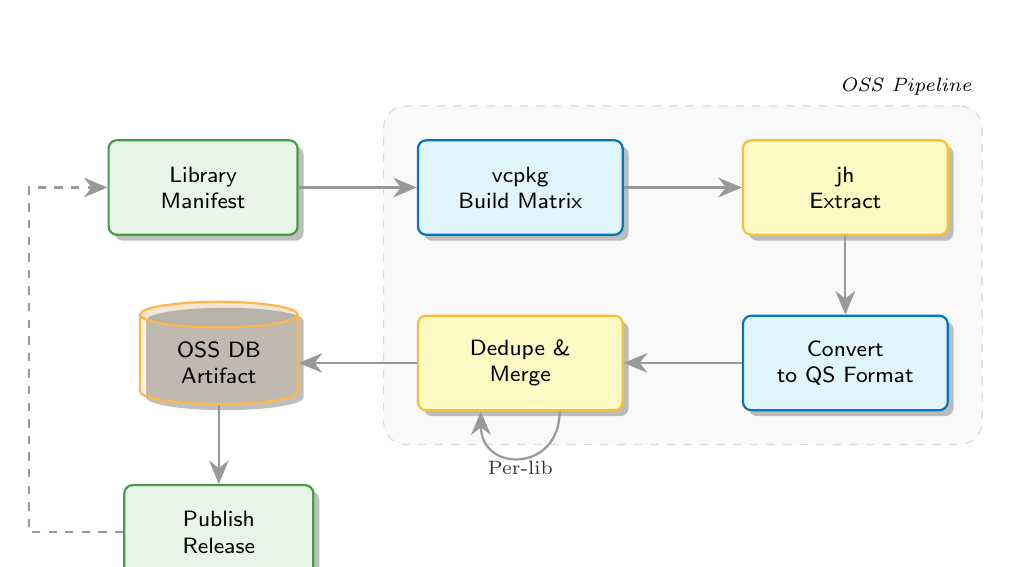
\begin{tikzpicture}[node distance=1cm and 1.5cm]
        \node[dataNode] (manifest) {Library\\Manifest};
        \node[opNode, right=of manifest] (build) {vcpkg\\Build Matrix};
        \node[procNode, right=of build] (jh) {jh\\Extract};
        \node[opNode, below=of jh] (convert) {Convert\\to QS Format};
        \node[procNode, left=of convert] (merge) {Dedupe \&\\Merge};
        \node[memNode, left=of merge] (artifact) {OSS DB\\Artifact};

        \node[dataNode, below=of artifact] (publish) {Publish\\Release};

        \begin{scope}[on background layer]
            \node[group, fit=(build)(jh)(convert)(merge)] (pipeline) {};
            \node[above left] at (pipeline.north east) {\scriptsize \textit{OSS Pipeline}};
        \end{scope}

        \draw[arrow] (manifest) -- (build);
        \draw[arrow] (build) -- (jh);
        \draw[arrow] (jh) -- (convert);
        \draw[arrow] (convert) -- (merge);
        \draw[arrow] (merge) -- (artifact);
        \draw[arrow] (artifact) -- (publish);
        \draw[arrow] ([xshift=0.5cm]merge.south) to[out=270, in=270, looseness=2] node[midway, below, edgeLabel] {Per-lib} ([xshift=-0.5cm]merge.south);
        \draw[arrow, dashed] (publish) -| ([xshift=-1cm]manifest.west) -- (manifest.west);
    \end{tikzpicture}
    \caption{Automatic tag database construction pipeline for OSS libraries.}
    \end{figure}

    \textbf{Deliverables:} A merge ready QS codebase with both small UX improvements and a stable, efficient pipeline to update string tagging databases, specifcally the \texttt{\#oss} database.

\end{itemize}

\subsubsection*{Integration of QS features into FLOSS}
\phantomsection
\addcontentsline{toc}{subsubsection}{Integration of QS features into FLOSS}

I propose a slice-based incremental method to slowly introduce the features without causing any breaking changes in \texttt{master}. We will create simple classes and methods initially, then slowly increase their function as the features become more expansive.

\textbf{Slice 1}

\begin{itemize}
    \item Create \texttt{floss/qs\_integration.py} for modularity.
    \item Add an additional argument, \texttt{--quantum (default: False)} to toggle QS techniques.
    \item Add helper functions to translate between a \texttt{ResultDocument} of QS and FLOSS.
    \item (PE only) map the FLOSS strings to sections.
\end{itemize}

This first slice will serve as the baseline for future work, and will undoubtedly introduce many bugs. Its vital that we test extensively here so that we don't face bigger challenges down the line.

\textbf{Slice 2}

\begin{itemize}
    \item Add helpers to load tags and apply them to FLOSS \texttt{Tagger} $\to$ \texttt{QsTagResult} $\to$ \texttt{Merge into ResultDocument}.
    \item Copy the CI ymls from quantumstrand to master.
    \item Import all current DBs (\#expert, \#oss, \#common, \#winapi, etc.)
    \item Add tag filters (mute/hide/highlight) as CLI arguments.
\end{itemize}

This will take care of all tagging features and will establish the CI pipeline working along FLOSS's \texttt{build-db.yml}.

\textbf{Slice 3}

\begin{itemize}
    \item Port the \texttt{Structures} aspect of \texttt{compute\_pe\_layout} into \texttt{qs\_integration.py}.
    \item Begin adding ELF parser from Fred's fork through the \texttt{elffile} library.
    \item Add \texttt{StaticString}-only support for Mach-O executables.
    \item Compile a diverse corpus of test executables with varying properties such as stripped symbols, memory dumped (see User Feedback section for why), broken/padded samples, unusual malware samples, etc.
\end{itemize}

This is a all-in-one slice that introduces lots of smaller new features into various parts of the codebase. The eventual result will be a generic function accepting multiple sources, such as \texttt{analyze\_qs\_layout(..., formats=("pe","elf","macho"))}

\textbf{Slice 4}

This is meant as a buffer slice to work on smaller features like:

\begin{itemize}
    \item Discussing with the community and collecting general feedback of the previous slices.
    \item Finalizing whether to support more niche features such as shellcode support and language-specific tagging.
    \item Bug fixes, security patches, optimizations for previous code that was overlooked to just get it ported, etc.
    \item Begin writing documentation based on discussions with mentors (see the Documentation section for more details).
\end{itemize}

\begin{figure}[H]
\centering
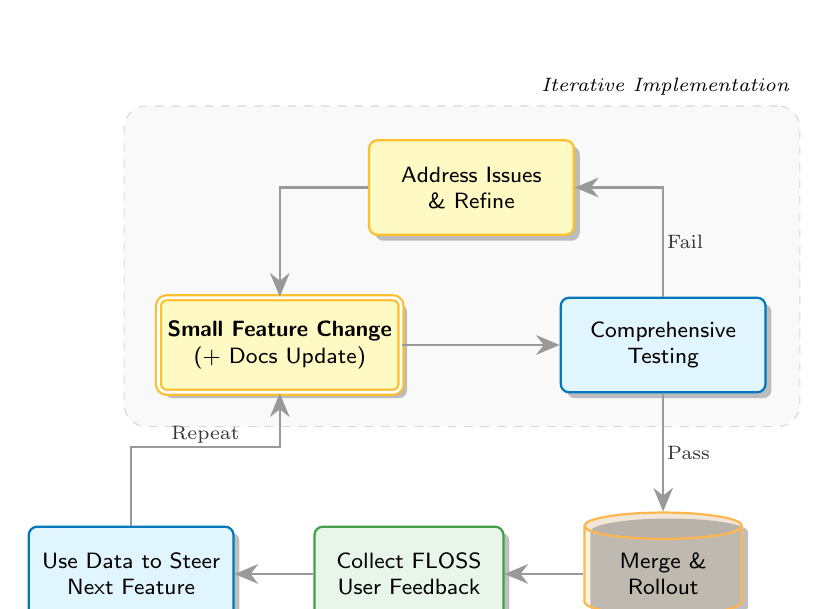
\begin{tikzpicture}[node distance=1.5cm and 2cm]
    \node[procNode, double, double distance=1pt] (dev) {\textbf{Small Feature Change}\\(+ Docs Update)};
    \node[opNode, right=of dev] (test) {Comprehensive\\Testing};
    \node[procNode] (fix) at ($(dev)!0.5!(test) + (0, 2cm)$) {Address Issues\\\& Refine};
    \node[memNode, below=1.5cm of test] (merge) {Merge \&\\Rollout};
    \node[dataNode, left=1cm of merge] (feedback) {Collect FLOSS\\User Feedback};
    \node[opNode, left=1cm of feedback] (steer) {Use Data to Steer\\Next Feature};
    \draw[arrow] (dev) -- (test);
    % Fail Loop
    \draw[arrow] (test.north) |- node[pos=0.25, right, edgeLabel] {Fail} (fix.east);
    \draw[arrow] (fix.west) -| (dev.north);
    % Pass
    \draw[arrow] (test.south) -- node[midway, right, edgeLabel] {Pass} (merge.north);
    % Rollout and Feedback
    \draw[arrow] (merge.west) -- (feedback.east);
    \draw[arrow] (feedback.west) -- (steer.east);
    % Repeat Loop
    \draw[arrow] (steer.north) -- ++(0, 1cm) -| node[near start, above, edgeLabel] {Repeat} (dev.south);
    \begin{scope}[on background layer]
        \node[group, fit=(dev)(test)(fix)] (devloop) {};
        \node[above left] at (devloop.north east) {\scriptsize \textit{Iterative Implementation}};
    \end{scope}
\end{tikzpicture}
\caption{Slice-based incremental method and community feedback loop.}
\end{figure}

\textbf{Merged FLOSS + QS JSON}

To keep this explicit and testable, here is an example of the merged output. When the \texttt{quantum} flag is enabled, the output JSON will follow this shape, with existing FLOSS fields preserved and optional \texttt{qs\_*} enrichments added.
\texttt{qs\_layout} stores structural hierarchy only; per-string QS metadata (\texttt{qs\_tags}, \texttt{qs\_section}, etc) is stored on each FLOSS string object.

\begin{lstlisting}[language=json]
{
  "analysis": {
    "enable_static_strings": true
  },
  "metadata": {
    "file_path": "dotnet-hello.exe",
    "qs_enabled": true
  },
  "strings": {
    "static_strings": [
      {
        "string": "!This program cannot be run in DOS mode.",
        "offset": 77,
        "encoding": "ASCII",
        "qs_tags": ["#common"],
        "qs_structure": "header",
        "qs_section": "header"
      },
      {
        "string": "WriteLine",
        "offset": 1036,
        "encoding": "ASCII",
        "qs_tags": ["#common", "#msvc"],
        "qs_structure": "",
        "qs_section": ".text"
      }
    ]
  },
  "qs_layout": {
    "name": "pe",
    "offset": 0,
    "length": 3584,
    "children": [
      {
        "name": "header",
        "offset": 0,
        "length": 512
      },
      {
        "name": ".text",
        "offset": 512,
        "length": 1024
      }
    ]
  }
}
\end{lstlisting}

In practice, this merged format means:
\begin{itemize}
    \item Legacy FLOSS JSON tooling remains valid because the core roots are unchanged: \texttt{analysis}, \texttt{metadata}, \texttt{strings}.
    \item QS mode is indicated in metadata (e.g., \texttt{qs\_enabled: true}).
    \item Tags/structure/section are cleanly attached to each string via optional \texttt{qs\_tags}, \texttt{qs\_structure}, and \texttt{qs\_section}.
    \item \texttt{qs\_layout} provides the recursive section/resource tree for grouping and navigation in the viewer.
\end{itemize}

\textbf{Final Directory Structure of FLOSS}

\begin{minipage}{\textwidth}
\dirtree{%
.1 flare-floss/.
.2 floss/.
.3 main.py \DTcomment{adds the \texttt{--quantum} flag}.
.3 results.py \DTcomment{optional \texttt{qs\_*} fields (backward compatible)}.
.3 qs\_integration.py \DTcomment{new adapter entrypoints (layout + tags)}.
.3 qs\_types.py \DTcomment{new lightweight QS-compatible dataclasses/types}.
.3 render/.
.4 json.py \DTcomment{unchanged behavior, includes optional qs fields when present}.
.3 \dots.
.2 floss-viewer/ \DTcomment{FLOSS string viewer GUI ported from \texttt{qs-viewer}}.
.2 tests/.
.3 test\_qs\_integration\_cli.py \DTcomment{flag behavior}.
.3 test\_qs\_layout\_mapping.py \DTcomment{PE first, then ELF}.
.3 test\_qs\_tagging.py \DTcomment{winapi/common/OSS/expert tagging}.
.3 test\_qs\_visibility.py \DTcomment{hide/mute/highlight rules}.
.3 test\_results\_schema\_compat.py \DTcomment{old/new JSON load compatibility}.
.2 doc/.
.3 quantumstrand.md \DTcomment{architecture + rollout notes}.
.2 .github/workflows/.
.3 (existing CI + QS integration test jobs).
.3 build-db.yml.
}
\end{minipage}

\textbf{Deliverables:} A merged \texttt{master} branch integrating core QS features (section mapping, tagging, filtering) with existing FLOSS functionality, backed by comprehensive tests. It also includes a checked-in JSON Schema and compatibility tests ensuring seamless GUI ingestion of both legacy and QS-augmented formats.

\pagebreak

\subsubsection*{Creating an interactive GUI to display strings}
\phantomsection
\addcontentsline{toc}{subsubsection}{Creating an interactive GUI to display strings}

Currently the baseline GUI for QS which I've improved is below:

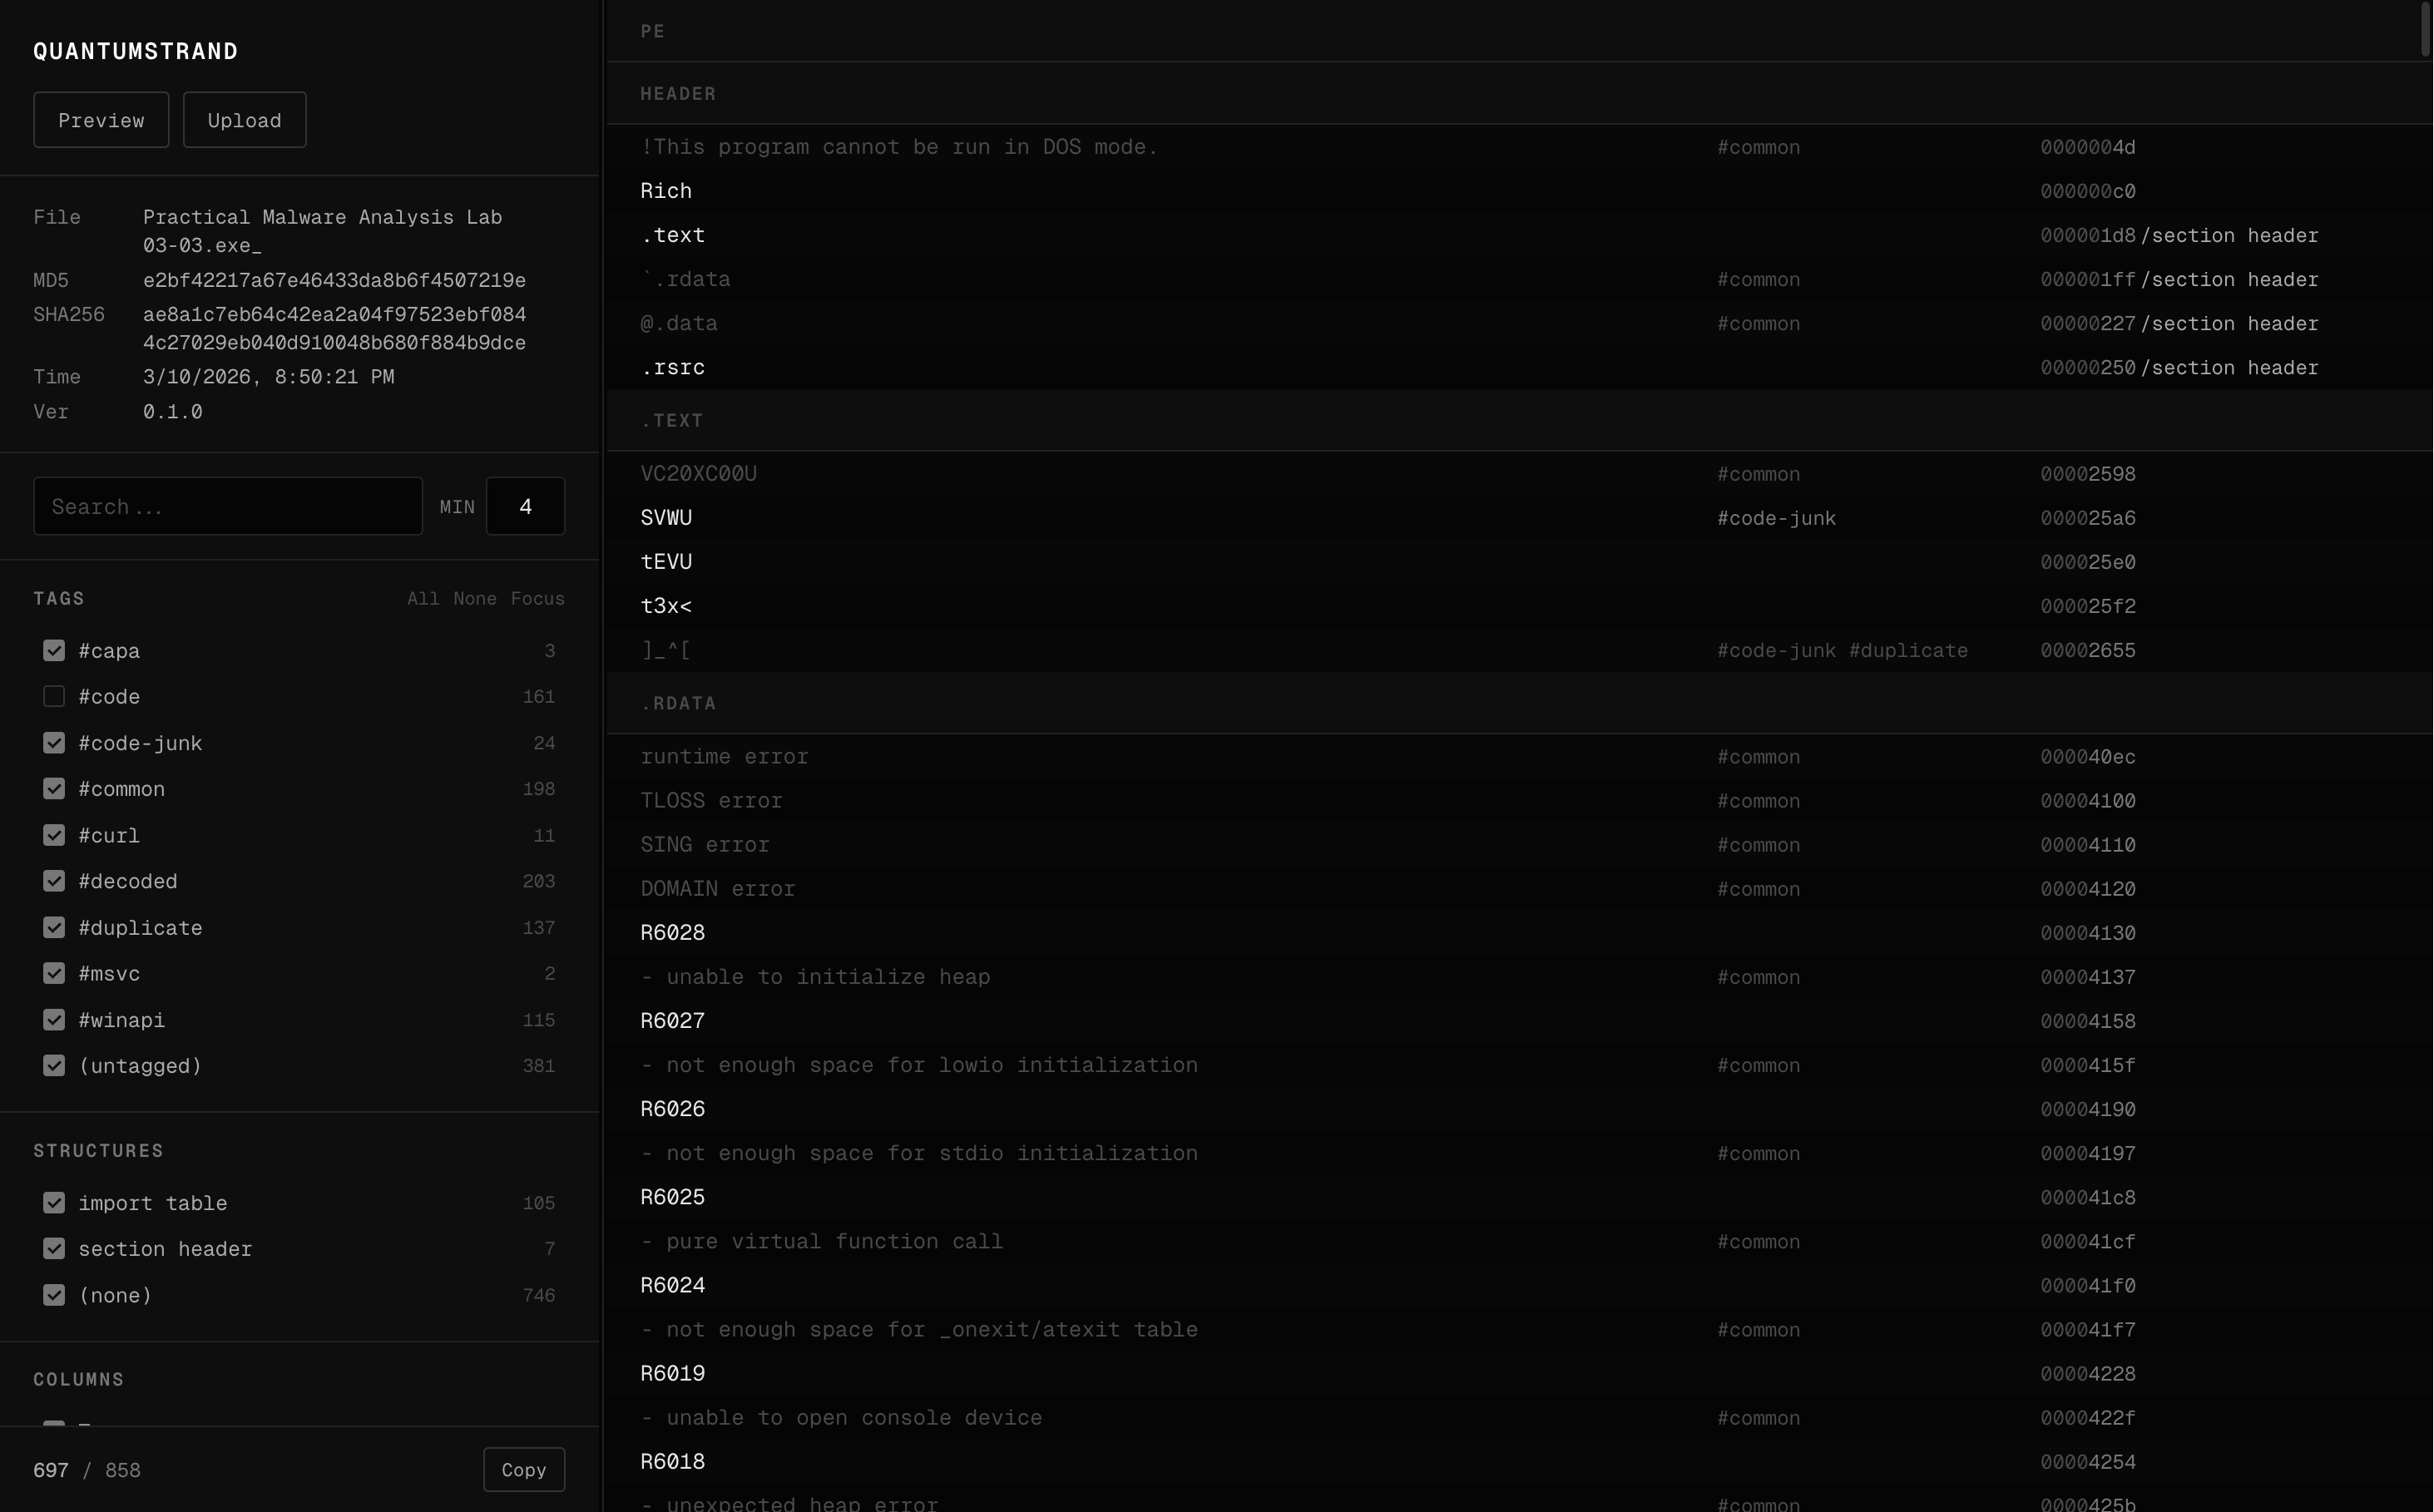
\includegraphics[width=1.0\textwidth]{assets/qs-viewer.png}

The link to my branch is here: \textcolor{RoyalBlue}{\href{https://github.com/vee1e/flare-floss/tree/qs-viewer-enhance}{\textbf{qs-viewer-enhance}}}. It contains a sidebar for tag filtering, sample metadata and other interactive options. The right 80\% is purely for viewing strings, with the output translated 1-to-1 from the CLI QS output.

The current features it supports are limited:

\begin{itemize}
    \item Filtering of tags and tag categories (``All'', ``None'', ``Focus'').
    \item Exact, linear searching of strings by content or length.
    \item Viewing of the sample metadata such as name, path, hashes, and date/time.
    \item Copying of selected and filtered strings to clipboard.
\end{itemize}

I propose a few crucial improvements and required features to add to this as it becomes FLOSS-native:

\begin{itemize}
    \item Merge FLOSS and QS output schema. Refer to \textbf{Merged FLOSS + QS JSON} above.
    \item Then we add the string metadata shown in native FLOSS CLI output. This is a simplified example output FLOSS produces:

        \begin{lstlisting}[language=yaml]
FLARE FLOSS RESULTS (version 3.1.1)
+------------------------+---------------------------+
| file path              | dotnet-hello.exe          |
| identified language    | dotnet (version unknown)  |
| static strings         | 57 (1028 characters)      |
+------------------------+---------------------------+
FLOSS Static Strings: ASCII and UTF-16 LE
Other FLOSS strings, such as stack, tight and decoded\end{lstlisting}
       Strings will be sorted section-wise as in the example, but with a clear indicator of whether they're static, stack, tight or decoded, and also language-based. The sidebar will expand to include FLOSS exclusive metadata such as identified language and number of extracted strings of each type.
    \item For QS specific enhancements, there are several good ideas already given in the \href{https://github.com/mandiant/flare-floss/issues?q=is\%3Aissue\%20state\%3Aopen\%20label\%3AQS\%2Fui}{\textbf{\textcolor{ForestGreen}{QS/ui}}} label. Some such as consolidation of adjacent tags have been accomplished in the CLI already and can be ported to the GUI.
    \item Implement other QoL enhancements such as custom tagging, selection of strings, and exporting the filtered/selected JSON.
    \item Add fuzzy search for the strings using an appropriate library such as Fuse.JS.
    \item Create features for tagging metadata. Hovering over a tag will give you more information pertaining to what the tag db actually does, what other strings it consists of, and in cases like \#expert, CAPA-aware metadata such as the rule name and the ATT\&CK technique associated with it. As the DBs are inside the repository itself, performance and latency won't be a major issue.
    \item After implementing these features, move to addressing performance bottlenecks. Loading a JSON with over 100,000 strings greatly impacts the performance in load times, filtering and general scrolling and viewing. For this we'll implement optimizations such as lazy loading and virtual scrolling.
    \item Deploy this to a live website so that a user doesn't need to install the entire FLOSS suite to just view data that he already has. Since this consists of only a frontend, GitHub pages is the most suitable option.
\end{itemize}

The current \texttt{qs-viewer} is a React app with Vite as a bundler. I will keep the current stack as-is, but move the runtime from NPM to Bun for faster builds.

As GUIs are subjective by their very nature, this will require a great deal of feedback to get right and will inevitably lead to conflicts. Listening to all stakeholders (contributors, mentors, and community) is significant here.

This frontend is organized into three simple, modular layers, \textbf{Ingestion}, \textbf{Data} and \textbf{Presentation}, all in \texttt{floss-viewer/}.

The ingestion step loads the FLOSS JSON, validates it, and normalizes missing fields into one consistent \texttt{ViewerDocument} structure; this will be best split across modules such as \texttt{ingest/loadFile.ts}, \texttt{validateFlossDocument.ts}, and \texttt{normalizeDocument.ts}.

From there, the main state, search and filter parts stay separate from rendering. The \texttt{Viewer} state holds search text, selected tags, structures, types, and layout toggles, while lazy loading and indexed lookups compute the active result set efficiently for large files.

The frontend consumes the output given by FLOSS JSON in \texttt{floss-viewer/} to render the sidebar, grouped string list, and export actions. This keeps loading, filtering, and rendering clearly separated and makes the viewer easier to extend without coupling UI components to FLOSS internals.

Unit and Integration Tests will be written to validate all features such as normalization, search, filter, and a complete pipeline from JSON to export/copy.

\begin{figure}[H]
\centering
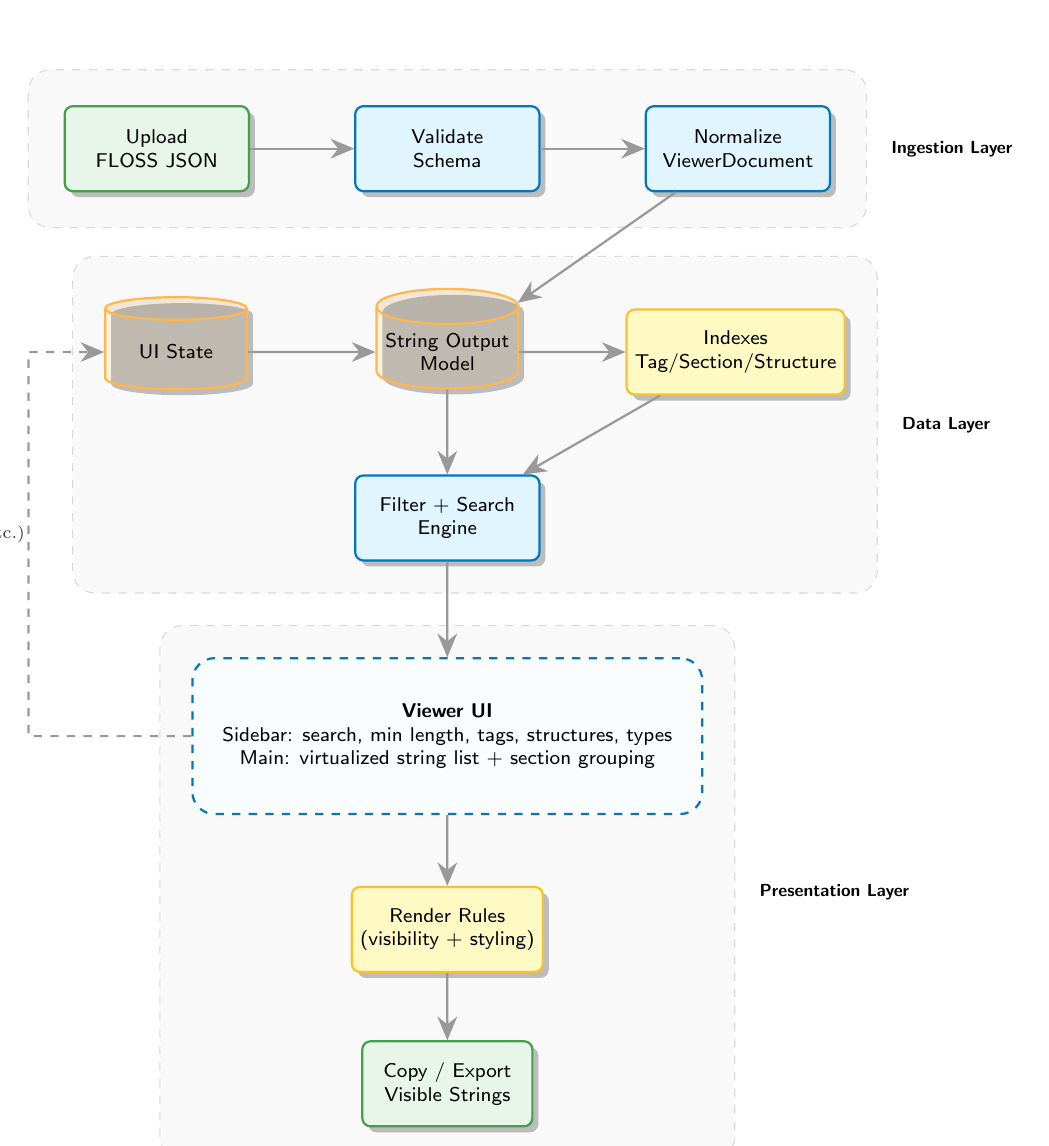
\begin{tikzpicture}[node distance=0.9cm and 1.0cm, scale=0.9, transform shape]
\node[opNode] (validate) {Validate\\Schema};
\node[dataNode, minimum width=2.6cm] (upload) at ([xshift=-4.1cm]validate.center) {Upload\\FLOSS JSON};
\node[opNode] (normalize) at ([xshift=4.1cm]validate.center) {Normalize\\ViewerDocument};
\node[memNode, below=1.35cm of validate] (model) {String Output\\Model};
\node[memNode, left=1.8cm of model] (state) {UI State};
\node[procNode, right=1.5cm of model] (index) {Indexes\\Tag/Section/Structure};
\node[opNode, below=1.2cm of model] (filter) {Filter + Search\\Engine};
\node[kernelBox, below=1.35cm of filter, minimum width=6.2cm, minimum height=2.2cm] (ui) {
\textbf{Viewer UI}\\
Sidebar: search, min length, tags, structures, types\\
Main: virtualized string list + section grouping
};
\node[procNode, below=1.0cm of ui] (render) {Render Rules\\(visibility + styling)};
\node[dataNode, below=0.95cm of render] (actions) {Copy / Export\\Visible Strings};
\draw[arrow] (upload) -- (validate);
\draw[arrow] (validate) -- (normalize);
\draw[arrow] (normalize) -- (model);
\draw[arrow] (state) -- (model);
\draw[arrow] (model) -- (index);
\draw[arrow] (index) -- (filter);
\draw[arrow] (model) -- (filter);
\draw[arrow] (filter) -- (ui);
\draw[arrow] (ui) -- (render);
\draw[arrow] (render) -- (actions);
\coordinate (ucStart) at ([xshift=-2.3cm]ui.west);
\coordinate (ucEnd) at (ucStart |- state.west);
\draw[arrow, dashed, overlay] (ui.west) -- (ucStart) -- node[edgeLabel, left, pos=0.55] {user changes\\(search, filters, etc.)} (ucEnd) -- (state.west);
\coordinate (g1L) at ([xshift=-5.4cm]validate.center);
\coordinate (g1R) at ([xshift=5.4cm]validate.center);
\coordinate (g2L) at ([xshift=-3.2cm]model.center);
\coordinate (g2R) at ([xshift=3.2cm]model.center);
\coordinate (g3L) at ([xshift=-3.5cm]ui.center);
\coordinate (g3R) at ([xshift=3.5cm]ui.center);
\begin{scope}[on background layer]
\node[group, fit=(g1L)(g1R)(upload)(validate)(normalize), inner sep=0.45cm] (g1) {};
\node[group, fit=(g2L)(g2R)(state)(model)(index)(filter), inner sep=0.4cm] (g2) {};
\node[group, fit=(g3L)(g3R)(ui)(render)(actions), inner sep=0.4cm] (g3) {};
\node[font=\sffamily\bfseries\scriptsize, anchor=west] at ([xshift=0.22cm]g1.east) {Ingestion Layer};
\node[font=\sffamily\bfseries\scriptsize, anchor=west] at ([xshift=0.22cm]g2.east) {Data Layer};
\node[font=\sffamily\bfseries\scriptsize, anchor=west] at ([xshift=0.22cm]g3.east) {Presentation Layer};
\end{scope}
\end{tikzpicture}
\caption{Frontend viewer architecture}
\end{figure}

\begin{center}
\begin{minipage}{\textwidth}
\dirtree{%
.1 floss-viewer/.
.2 package.json \DTcomment{frontend dependencies and scripts}.
.2 vite.config.ts \DTcomment{Vite config}.
.2 index.html \DTcomment{app entrypoint}.
.2 src/.
.3 main.tsx \DTcomment{bootstrap}.
.3 App.tsx \DTcomment{top-level app layout}.
.3 ingest/ \DTcomment{file loading, validation, normalization}.
.3 model/ \DTcomment{canonical viewer document types}.
.3 state/ \DTcomment{viewer state and selectors}.
.3 query/ \DTcomment{indexes, filtering, search}.
.3 components/ \DTcomment{sidebar and viewer components}.
.3 render/ \DTcomment{visibility and style rules}.
.3 export/ \DTcomment{copy and export helpers}.
.3 styles/ \DTcomment{shared viewer styling}.
.2 tests/ \DTcomment{all testing infra}.
}
\end{minipage}
\captionof{figure}{Planned high-level directory structure for the FLOSS viewer frontend.}
\end{center}

\textbf{Deliverables:} An intuitive, full-featured and well designed deployed GUI interface that allows exploration of any aspect of the strings exposed by FLOSS and QS.

\newpage
\subsubsection*{Documentation}
\phantomsection
\addcontentsline{toc}{subsubsection}{Documentation}

The final but equally important part. For this we'll use a single file \texttt{doc/quantumstrand.md}.

This will include the following details

\begin{itemize}
    \item The theory and philosophy behind QS and why it serves crucial part of malware string analysis, essentially the \texttt{theory.md}.
    \item Various features of QS, and what methods and APIs are exposed for it, and how to extend features or create new ones.
    \item Reports of the various libraries used and the algorithms used to process the data generated from them (particularly for string tagging).
    \item A technical description of the GUI along with screenshots demonstrating the features \textbf{(will go inside the main FLOSS \texttt{usage.md})}
\end{itemize}

Parallel to this, I will also work on a blog post detailing my GSoC journey to give the perspective of a student QS developer and would serve as a good reference for future contributors.

\textbf{Deliverables:} A comprehensive technical document detailing the important parts needed for further development of the project.

\subsection*{Weekly timeline}
\phantomsection
\addcontentsline{toc}{subsection}{Weekly timeline}

The work is divided into four phases:

\colorbox{ForestGreen!10}{\textbf{Phase 1}} covers improving existing QS functionality and stabilizing missing pieces.

\colorbox{Cerulean!10}{\textbf{Phase 2}} focuses on integrating those capabilities into FLOSS.

\colorbox{Apricot!18}{\textbf{Phase 3}} is dedicated to GUI development in \texttt{floss-viewer/}.

\colorbox{Orchid!10}{\textbf{Phase 4}} is reserved for documentation, cleanup, and final polish.

\renewcommand{\arraystretch}{1.25}
{\scriptsize
\begin{longtable}{|>{\centering\arraybackslash}m{1.45in}|>{\centering\arraybackslash}m{0.95in}|>{\raggedright\arraybackslash}m{2.55in}|>{\raggedright\arraybackslash}m{1.05in}|}
\hline
\textbf{Period} & \textbf{Phase} & \textbf{Description} & \textbf{Deliverable} \\
\hline
\endfirsthead
\hline
\textbf{Period} & \textbf{Phase} & \textbf{Description} & \textbf{Deliverable} \\
\hline
\endhead
Community Bonding ~ ~ (May 1 -- May 24) & Prep & Deepen FLOSS codebase knowledge, study QS and FLOSS string decoding algorithms in detail, align with mentors and the community on project priorities, and fix any remaining setup or CI issues in the repo by merging 1-2 PRs before coding starts. & Finalized project plan and ready-to-code development environment. \\
\hline
\rowcolor{ForestGreen!10}
Week 1 (May 25 -- May 31) & Phase 1 & Start work on ELF and Mach-O section support in QS, focusing on layout handling and the initial parsing needed for both formats. & Initial ELF and Mach-O section support delivered with matching tests or validation samples. \\
\hline
\rowcolor{ForestGreen!10}
Week 2 (Jun 1 -- Jun 7) & Phase 1 & Migrate the string databases to Git LFS and perform local testing of the library build pipelines to validate the planned OSS database workflow before CI rollout. & Git LFS migration completed and local pipeline test results documented. \\
\hline
\rowcolor{ForestGreen!10}
Week 3 (Jun 8 -- Jun 14) & Phase 1 & Implement the first part of the CI pipeline for automated library builds, including workflow structure, build matrix setup, and artifact generation. & Initial CI workflow for library builds pushed and running. \\
\hline
\rowcolor{ForestGreen!10}
Week 4 (Jun 15 -- Jun 21) & Phase 1 & Complete and refine the CI automation by adding database conversion, dedupe/merge logic, and the remaining release-oriented workflow pieces. & End-to-end CI-driven database pipeline ready for integration and review. \\
\hline
\rowcolor{Cerulean!10}
Week 5 (Jun 22 -- Jun 28) & Phase 2 & Complete Slice 1 and the first tagging step of Slice 2 by adding \texttt{qs\_integration.py}, the \texttt{--quantum} flag, result translation helpers, PE section mapping, and the initial tag merge path. & Baseline FLOSS integration with initial tagging support. \\
\hline
\rowcolor{Cerulean!10}
Week 6 (Jun 29 -- Jul 5) & Phase 2 & Import the current string databases, add CLI tag filters for mute/hide/highlight behavior, and finish the tagging feature set against FLOSS CI. & Complete tagging integration validated by \texttt{build-db.yml}. \\
\hline
\rowcolor{Goldenrod!18}
\multicolumn{4}{|c|}{\textbf{Midterm Evaluation} (\textbf{July 10, 2026})} \\
\hline
\rowcolor{Cerulean!10}
Week 7 (Jul 6 -- Jul 12) & Phase 2 & Complete Slice 3 by adding structure support, beginning ELF parsing through \texttt{elffile}, adding scoped Mach-O support, and building a stronger executable test corpus. & Expanded multi-format integration with better structure coverage and tests. \\
\hline
\rowcolor{Cerulean!10}
Week 8 (Jul 13 -- Jul 19) & Phase 2 & Use this week to collect feedback, clean up rough edges, and make final decisions on what should or should not be included in scope. & Stable and reviewable QS integration phase. \\
\hline
\rowcolor{Apricot!18}
Week 9 (Jul 20 -- Jul 26) & Phase 3 & Begin the GUI phase by setting up the viewer structure and migrating the frontend from QS to FLOSS output JSON schema. & Working frontend foundation with FLOSS JSON support. \\
\hline
\rowcolor{Apricot!18}
Week 10 (Jul 27 -- Aug 2) & Phase 3 & Implement the main viewer interface, including sidebar controls, grouped rendering, virtualized string lists, and core search/filter behavior. & Usable viewer MVP with core interaction flows. \\
\hline
\rowcolor{Apricot!18}
Week 11 (Aug 3 -- Aug 9) & Phase 3 & Finish advanced GUI features such as fuzzy search, richer tag metadata interaction, copy/export actions, and performance tuning for large JSON inputs. & Feature-complete GUI ready for final polish. \\
\hline
\rowcolor{Orchid!10}
Week 12 (Aug 10 -- Aug 16) & Phase 4 & Complete \texttt{doc/quantumstrand.md}, usage-oriented documentation, screenshots, final cleanup, and any remaining polish before submission. & Final documentation and submission-ready project state. \\
\hline
\rowcolor{Goldenrod!25}
\multicolumn{4}{|c|}{\textbf{Final Submission} (\textbf{August 24, 2026})} \\
\hline
\end{longtable}
}

\newpage
\section*{Future Plans}
\phantomsection
\addcontentsline{toc}{section}{Future Plans}

If I am selected for the program, I would like to continue contributing to the FLOSS project post-GSoC by focusing on the long-term maintainability and expansion of FLOSS. My post-program roadmap includes creating comprehensive Doxygen documentation for the entire FLOSS codebase to streamline contributor onboarding, researching language-specific string extraction heuristics for niche languages like Nim and Zig to keep pace with evolving malware trends, and conducting a feasibility study into migrating the disassembly backend from Vivisect to alternatives such as Capstone or \texttt{idalib} for improved performance.

\section*{Availability}
\phantomsection
\addcontentsline{toc}{section}{Availability}

I am almost entirely free for the entire duration of the program, from Week 1 through the final evaluation period. I have no other academic, internship, or professional commitments during this time and can dedicate 20--35 hours per week consistently to this project, totaling approximately 350 hours across the coding period (12 weeks), which matches the expected project effort.

I have my semester final exams from May 2 -- May 19 during the Community Bonding period, however I will remain active in the Org regardless.

My regular working window will be in the evening to late night, typically 18:00--00:00 IST (13:30--19:30 CET), giving me a good 5--6 hours a day for collaboration, implementation, and mentor feedback.

\section*{AI Disclosure}
\phantomsection
\addcontentsline{toc}{section}{AI Disclosure}

AI was used to proofread the text and fix grammatical errors and issues. It was also used in refining the diagrams and table formatting.
Besides this, all text content and code is entirely human-typed, and I take full responsibility for any code I write.
This is fully in line with Mandiant's \href{https://github.com/mandiant/flare-gsoc/blob/2026/doc/contributor-guidance.md#ai-tooling-guidance}{\textbf{AI tooling guidance}} policy.

\end{document}
